\section{Experiment Results}
\subsection{Evaluation Metrics}
 Recall the following definition of precision recall curve. Given a test data set of size $n$, each with $m$ features, $\{(f_{ij}, p_i)\}_{i \in [n], j \in [m]}$, a binary classifier (such as SVM, logistic regression, gbdt, etc) typically outputs a score for each record $p((f_{i1}, \ldots, f_{im}))$.  The records are classified as positive or negative based on whether the score exceeds a fixed threshold $\lambda$ or not. 
\begin{definition}
Given a sequence of score-label pairs $(s_i,\ell_i)$, $1 \le i \le n$, sorted by first component then second, such that $s_i \le s_j$ for $i< j$, and $\ell_i \in \{-1,+1\}$, the Precision-Recall (PR) curve is the linear interpolation of the set of points $(r_i,p_i)$, with flat extrapolation from the leftmost point to the $y$-axis, where $p_i = \frac{\rm{TP}_i}{\rm{TP}_i + \rm{FP}_i}$ is the precision at position $i$, and $r_i =\frac{\rm{TP}_i}{\rm{TP}_i + \rm{FN}_i}$ is the recall at position $i$. Here we define
\begin{itemize}
\item $\rm{TP}_i := |\{j \le i: \ell_j =+1\}|$, the number of truelabels above position $i$ (true positives),
\item $\rm{FP}_i := |\{j \le i: \ell_j =-1\}|$, the number of false labels above position $i$(false positives),
\item $\rm{FN}_i := |\{j > i: \ell_j = +1\}|$, the number of true labels below position $i$(false negatives).
\end{itemize}
\end{definition}

\begin{definition}
The Receiver Operating Characteristic (ROC) curve is defined similarly, replacing $(r_i,p_i)$ with $(f_i, t_i)$, where $f_i = \frac{\rm{FP}_i}{\rm{FP}_i + \rm{TN}_i}$ is the false positive rate at position $i$ and $t_i = \frac{\rm{TP}_i}{\rm{TP}_i + \rm{FN}_i}$ is the true positive rate. 
\end{definition}

\begin{definition}
The Area Under Curve (AUC) can be defined for either Precision-Recall curve or the ROC curve as above. If we parametrize the curve as the graph of a function $\gamma:[0,1] \to [0,1]$, the AUC is defined by
\begin{align*}
\rm{AUC} = \int_0^1 \gamma(t) dt.
\end{align*}
Note that the x-coordinates of both curves attains the maximum value of $1$, since at position $i = n$, $\rm{TN}_i = \rm{FN}_i = 0$ by definition. It is possible in theory that the x-coordinates to hit $0$, precisely when the top ranked article has a negative label. However in practical situations there is always a gap between the left most point and the y-axis, which can be addressed with any reasonable extrapolation scheme. Here we choose flat extrapolation to facilitate probabilistic calculations.

Since the curves are piecewise linear, given by linear interpolation of a finite set of $n$ points, the integral can be easily and exactly computed using the Trapezoid rule.
\end{definition}

For phase 0 stream filter, we use precision-recall AUC as the principle measure of performance. The labels are generated using either heuristic methodology based on production filter in combination with unique user click statistics, or editorial judgment. The latter data is sparse but has high fidelity. AUC of $1$ corresponds to the perfect situation where all the positively labeled articles are ranked higher than the negatively labeled ones. This does not mean that a threshold is not necessary, but only that a perfect threshold is feasible, and that for any threshold level, the total number of misclassifications is optimal (minimal) among all rankings. 

For phase 1 and 2, we use primary AUC under the ROC curve, based on the user click feedback. Thus a clicked article $d$ by a user $u$ is considered a positive example, whereas the rest are negative examples. This is an appropriate metric here because the end goal here is ranking. AUC for ROC can be seen as a specialization of a family of permutation statistics, with notable examples such as Kendall's tau, that measures the number of pairs of records whose relative order is reversed compared to the true ranking. It is also conveniently agnostic to the ratio between the numbers of positive and negative labels. 



ROC curve is always monotone non-decreasing, which is easily seen by rewriting $t_i = \frac{1}{1 + \rm{FN}_i / \rm{TP}_i}$ and $f_i = \frac{1}{1 + \rm{TN}_i / \rm{FP}_i}$, and noticing the subfractions are both monotone in $i$. The PR curve however can be highly non-montone in general, since the quantity $\rm{FP}_i / \rm{TP}_i$ has no monotonicity in general. An easy example is given by $n-1$ positively labeled data and a single negatively labeled one: in this case the curve starts off with $p_i =1$ until the index reaches the negatively labeled datum, at which point the curve drops to $\frac{i-1}{i}$, which however is an increasing function in $i$. In a sense, the more monotone the PR curve, the better it is from predicting completely randomly.


It is important also to note that while the AUC for ROC curve always has a mean of $0.5$ under uniform ranking, easily proved using the equivalence with Mann-Whitney-Wilcoxon statistics, provided there is at least one positive example and one negative example,  the AUC for the PR curve has a uniform baseline distribution that depends on the exact ratio between positive and negative examples. Again with the example of one negatively labeled datum, where the predicted rank of the negative example is uniformly random, then using flat extrapolation to the left, the expected AUC for PR curve is given by 
\begin{align*}
\frac{1}{n} \sum_{k=1}^n [\frac{k}{n} + \sum_{i=k+1}^n \frac{i-1}{in}] = 1 + o(1).
\end{align*}
In general it's easy to show (by considering pointwise average) that the average AUC is given by $P/n$, where $P$ is the total number of positively labeled examples. This is especially important for the stream filter evaluation, since there tends to be many more negative examples than positive ones. 

Finally to measure performance of phase 3 diversity algorithm, we introduce two additional metrics. The goal is to ensure maximal diversity among the top $k$ articles in the final ranking, while preserving the ranking from phase 2 as much as possible. The first metric thus measures the diversity directly, using the geometric interpretation of determinants as the volume of $k$-dimensional parallelopiped in an $m$-dimensional Euclidean positive orthant. Here $m$ is the number of features used in the diversity algorithm, namely YCT categories and wiki entities.
\begin{definition}
Given a set of ranked documents $d_i$,$ 1 \le i \le n$, each with $m$ features $\mathbf{f}_i = (f_{i1}, \ldots, f_{im})$,  we can define the top $k$ Gram-determinantal diversity to be 
\begin{align*}
d_k = \det (\langle \mathbf{f}_i , \mathbf{f}_j \rangle)_{1\le i,j \le k}
\end{align*}
The Determinantal Diversity (DD) curve is given by linear interpolation of the points $(k,d_k)$, $1 \le k \le n$. We can define similarly the AUC associated with the DD curve as before, with the technical caveat that the curve now span $[1,n]$ on the horizontal scale.
\end{definition}
 
To measure the amount of scrambling on phase 2 ranking due to phase 3 diversification, we use curves derived from two standards metrics: top $k$ Kendall's tau and top $k$ Mean Reciprocal Rank (MRR). To avoid unnecessary confusion, we will not look at AUC of these curves.

Kendall's tau can be seen as a generalization of AUC for ROC curve, where the set of labels is extended from a two-element set $\{-1,1\}$ to a set of $n$ elements, namely the rankings of all the objects. Formally we have
\begin{definition}
Given a predicted ranking sequence $\sigma(1), \ldots, \sigma(n)$, where $1,\ldots, n$ is the true ranking of the $n$ objects, the Kendall's tau of the prediction is given by
\begin{align*}
\rm{KT}(\sigma) = \mid \{ (i,j): 1 \le i< j \le n, \sigma(i) > \sigma(j) \} \mid / \binom{n}{2}.
\end{align*}
 Thus $\rm{KT}(\sigma)$ measures the number of ``pairwise disarrays". Under the normalization by $\binom{n}{2} = \frac{n(n-1)}{2}$, if $\sigma(i) = n-i+1$, we get the opposite ranking, with a KT score of exactly $1$.
\end{definition}

MRR is another standard metric in ranking literature. It penalizes mis-ranking for higher ranked articles more than that for lower ranked articles, which makes sense in the current semantic stream context.
\begin{definition}
Given a ranking of $n$ objects $\sigma(1),\ldots, \sigma(n)$, the top $k$ MRR is defined by
\begin{align*}
\rm{MRR}_k = \frac{1}{k}\sum_{i=1}^k \frac{1}{\sigma(i)}.
\end{align*}
Thus we prefer a top $k$ MRR curve that's monotone decreasing.
\end{definition}

\subsection{Test Results}

\subsubsection{Phase 0}

The precision-recall curve for the three streams (Sports, Finance, and NFL) are shown in figure 
% include AUC, features used, neg/pos data size, stream name, PR in caption 

\begin{figure}[H]
\centering
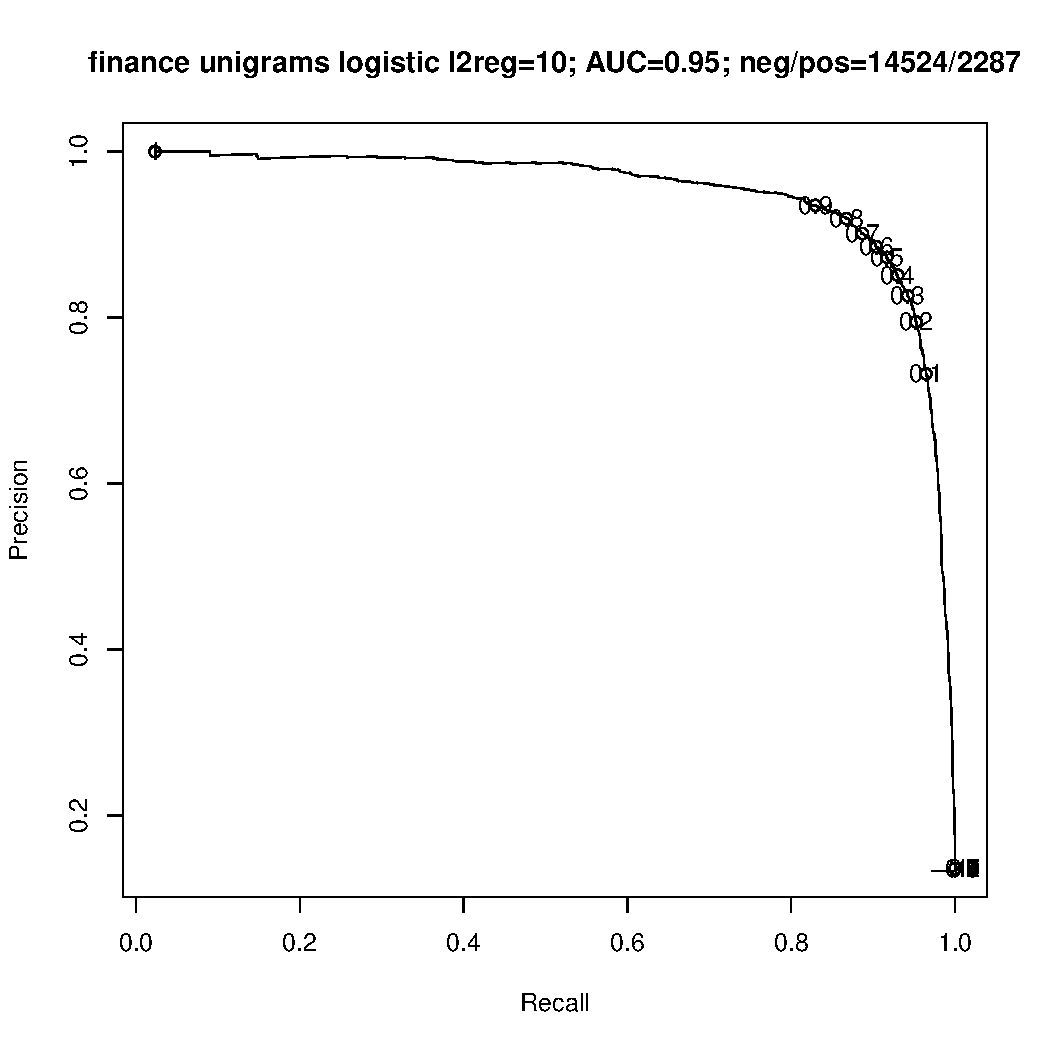
\includegraphics[scale=0.5]{PRcurve_fin.pdf}
\caption{"Finance Precision-Recall; unigram logistic , l2reg = 10; AUC = 0.95"}
\end{figure}

\begin{figure}[H]
\centering
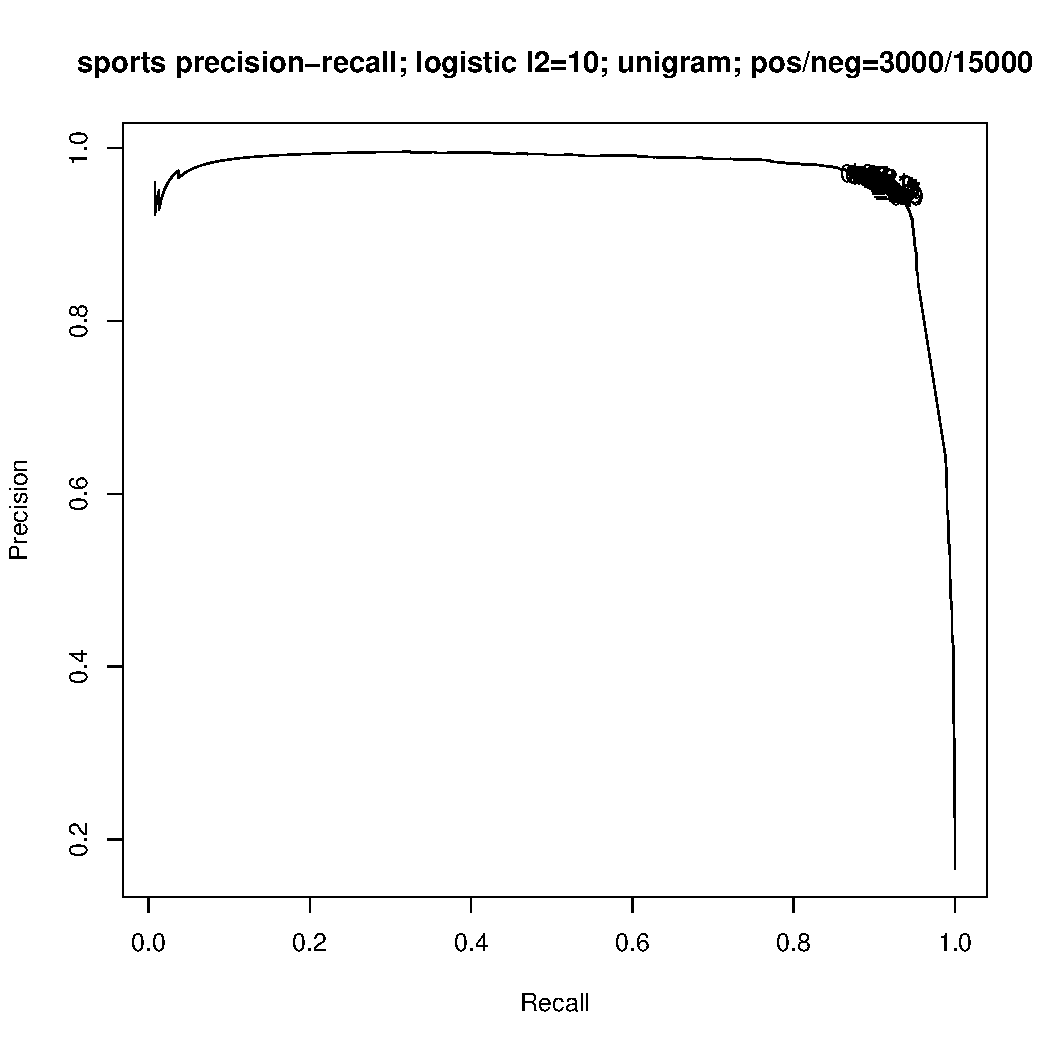
\includegraphics[scale=0.5]{PRcurve_spt.pdf}
\caption{"Sports Precision-Recall; unigram logistic , l2reg = 10; AUC = 0.97"}
\end{figure}

\begin{figure}[H]
\centering
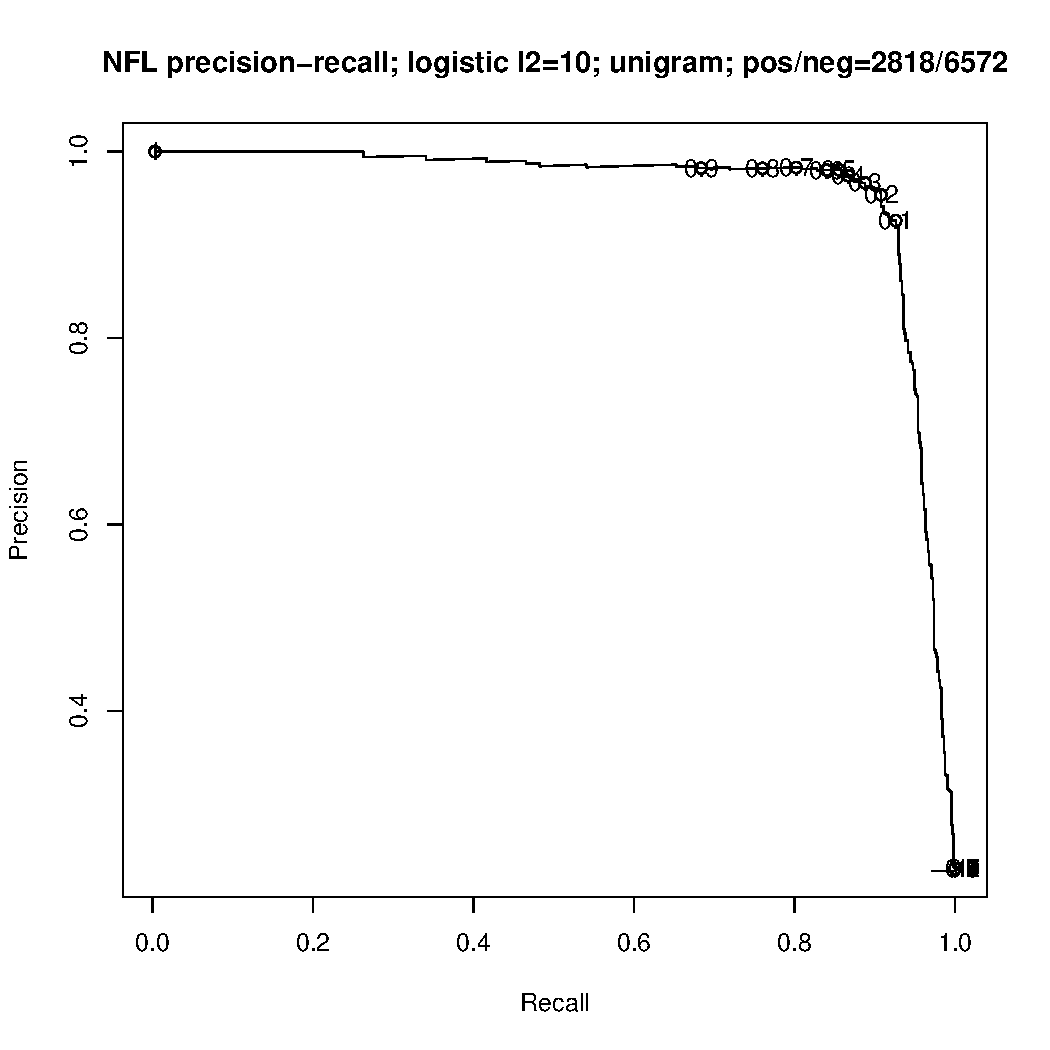
\includegraphics[scale=0.5]{PRcurve_nfl.pdf}
\caption{"NFL Precision-Recall; unigram logistic , l2reg = 10; AUC = 0.96"}
\end{figure}

Baseline classification error comparison:


\subsubsection{Phase 1}
Here we present the ROC AUC for Sports and Finance under four sets of training methodologies:
\begin{enumerate}
\item gmp only
\item flat dot-product (no SRQ) + gmp
\item SRQ + gmp
\item SRQ with negative pruning + gmp
\end{enumerate}


\subsubsection{Phase 2}

\subsubsection{Phase 3}

We illustrate the results with a single user session. 
\begin{figure}[H]
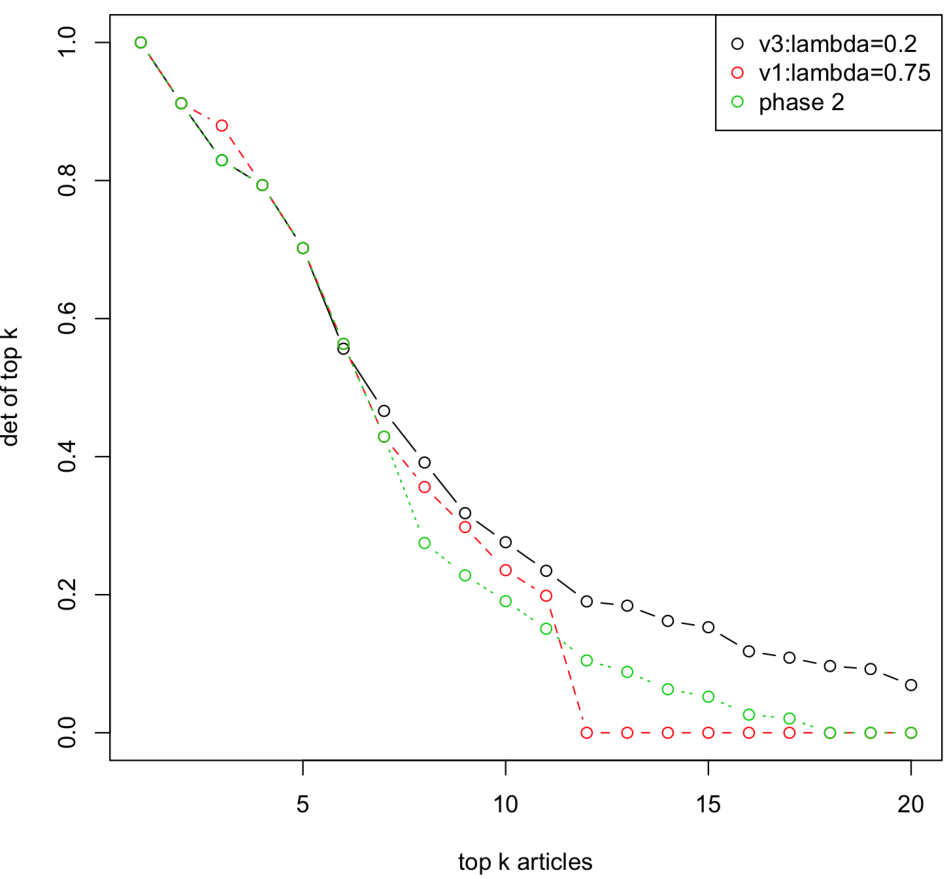
\includegraphics[scale=0.5]{DDcurve.pdf}
\caption{Determinantal Diversity Curve}
\end{figure}

\begin{figure}[H]
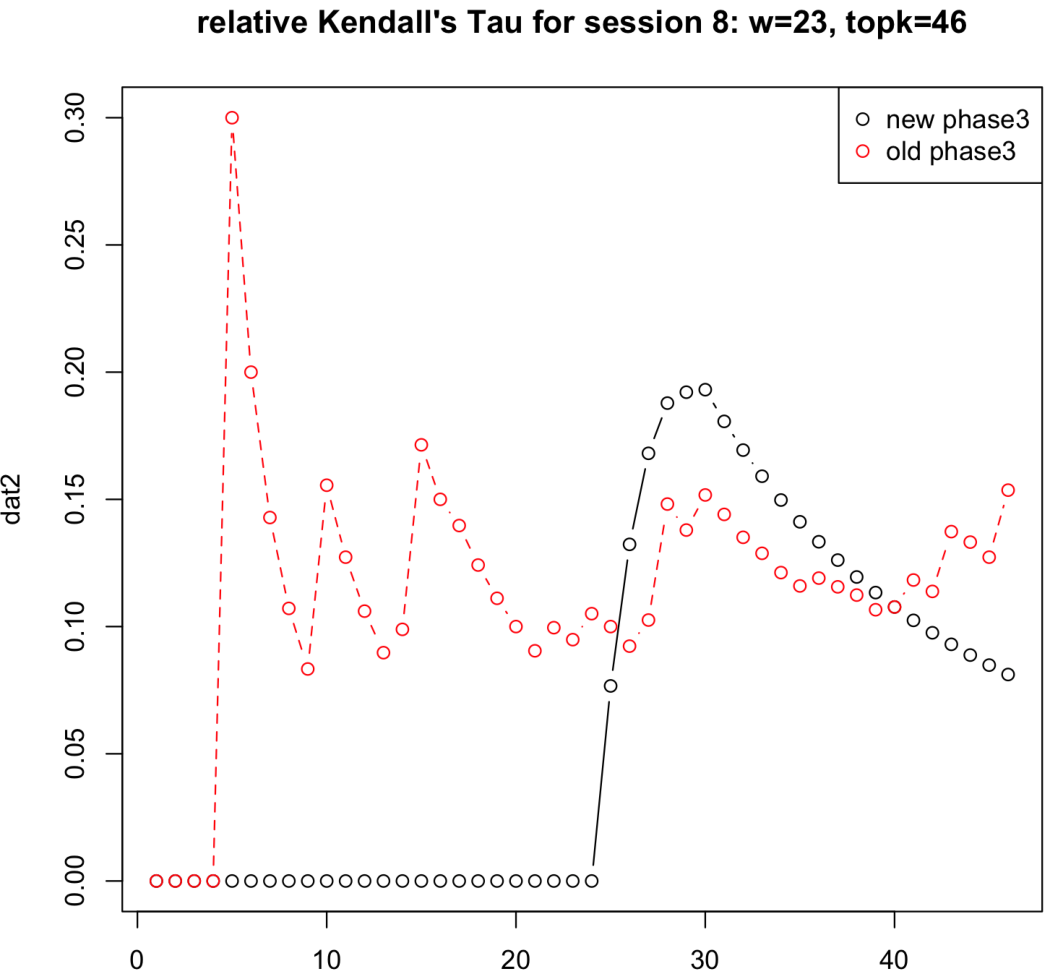
\includegraphics[scale=0.5]{KTcurve.pdf}
\caption{Kendall's Tau Curve}
\end{figure}

It's clear that the diversity algorithm v3 performs the best in comparison with v1 (so-called MMR approach) or with no diversity at all, consistently across all top k positions, with only one except at position 3. More importantly, by design v3 preserves the original order from phase 2 ranking up to the end of the first window limit. After the first window is exceeded, there is a momentary spike in top k Kendall tau metric, followed by rapid decrease to a level below that of v1. 


 

